\documentclass[12pt,dvipsnames]{article}

% Packages
%---------------------------------------------------------------------------------------------------
\usepackage[english]{babel}
\usepackage[svgnames]{xcolor}
\usepackage{natbib}
\usepackage{url}
\usepackage[utf8x]{inputenc}
\usepackage{amsmath}
\usepackage{verbatim}
\usepackage{graphicx}
\usepackage{parskip}
\usepackage{hyperref}
\usepackage{fancyhdr}
\usepackage{listings}
\usepackage{vmargin}
\setmarginsrb{2 cm}{1.5 cm}{2 cm}{1.5 cm}{1 cm}{1 cm}{1.5 cm}{1.5 cm}
\usepackage{minted}
\usepackage{hyperref}
\usepackage{float}
\usepackage{etoolbox}
\usepackage{tcolorbox}
\usepackage[
labelfont=sf,
hypcap=false,
format=hang,
width=\columnwidth
]{caption}

%Colors
%---------------------------------------------------------------------------------------------------
\definecolor{bg}{rgb}{0.95,0.95,0.95}
%---------------------------------------------------------------------------------------------------

% New commands
%---------------------------------------------------------------------------------------------------
\makeatletter
\patchcmd{\verbatim@input}{\@verbatim}{\scriptsize\@verbatim}{}{}
\makeatother

% Highlight some code
\newcommand{\Lcode}[1]{\texttt{\color{Blue}{#1}}}

% Shell command highlighting
\newcommand{\scom}[1]{
\vspace{0.2cm}
\begin{tcolorbox}
    \texttt{\color{Blue}{\$ #1}}
\end{tcolorbox}
}
% Multiple shell command highlighting
\newcommand{\mscom}[1]{
\vspace{0.2cm}
\begin{tcolorbox}
    \texttt{\color{Blue}{#1}}
\end{tcolorbox}
}
% Reference to code lines write only the line number
\newcommand{\refcode}[1]{\underline{line #1}}

% Caption for long listing (can be used also for short listing)
\newcommand{\Caption}[1]{\captionof{listing}{#1}\vspace{0.2cm}}
%---------------------------------------------------------------------------------------------------


%Definition of image path
%---------------------------------------------------------------------------------------------------
\graphicspath{{images/}}
%---------------------------------------------------------------------------------------------------


% Linking and reference style
%---------------------------------------------------------------------------------------------------
\hypersetup{
  colorlinks=true,
  linkcolor=SteelBlue,
  filecolor=IndianRed,
  urlcolor=IndianRed,
  citecolor=LightSlateGray,
  raiselinks=true
}

% Listing style
%---------------------------------------------------------------------------------------------------
\usemintedstyle{perldoc}
\setminted{
frame=lines,
bgcolor=bg,
fontsize=\footnotesize,
baselinestretch=1,
framesep=1mm,
linenos,
breaklines,
tabsize=1
}
%---------------------------------------------------------------------------------------------------




\begin{document}
%%%%%%%%%%%%%%%%%%%%%%%%%%%%%%%%%%%%%%%%%%%%%%%%%%%%%%%%%%%%%%%%%%%%%%%%%%%%%%%%
%%%%%%%%%%%%%%%%%%%%%%%%%%%%%%%%%%%%%%%%%%%%%%%%%%%%%%%%%%%%%%%%%%%%%%%%%%%%%%%%%%%%%%%%%%%
% cose da modificare ogni volta
%%%%%%%%%%%%%%%%%%%%%%%%%%%%%%%%%%%%%%%%%%%%%%%%%%%%%%%%%%%%%%%%%%%%%%%%%%%%%%%%%%%%%%%%%%%

\title{DNS Attacks and DNSSec securisation}													% Title
\author{Fabio Baldo}														% Author
\date{20/11/2020}														% Date

%%%%%%%%%%%%%%%%%%%%%%%%%%%%%%%%%%%%%%%%%%%%%%%%%%%%%%%%%%%%%%%%%%%%%%%%%%%%%%%%%%%%%%%%%%%


\makeatletter
\let\thetitle\@title
\let\theauthor\@author
\let\thedate\@date
\makeatother
\pagestyle{fancy}
\fancyhf{}
\rhead{\theauthor}
\lhead{\thetitle}
\cfoot{\thepage}
\newcommand{\mis}[3]{(#1 \pm #2) \ #3}
\newcommand{\misp}[3]{(#1 \#3 \pm #2}


%%%%%%%%%%%%%%%%%%%%%%%%%%%%%%%%%%%%%%%%%%%%%%%%%%%%%%%%%%%%%%%%%%%%%%%%%%%%%%%%%%%%%%%%%

\begin{titlepage}
	
    \begin{center}				
    \textsc{\LARGE HES-SO MSE}\\[2.0 cm]						% University Name
    
        \makebox[\textwidth]{
\includegraphics[width=\textwidth]{images/HES-SO-Haute-Ecole-Specialisee-de-Suisse-occidentale_ng_image_full.png}} % University Logo
        \vspace*{2.00 cm}
    
	\textsc{\Large Network security and architecture}\\[0.30 cm]		% Course Code
	\textsc{\Large S1-2021 }\\[0.5 cm]		%Anno accademico
	\textsc{\Large  }\\[0.5 cm] % Nome del Professore
	\rule{\linewidth}{0.2 mm} \\[0.4 cm]
	{ \huge \bfseries \thetitle \\ \small \thedate}\\
	\rule{\linewidth}{0.2 mm} \\[1.5 cm]
	
    	\begin{center}
    	    Fabio Baldo
    	\end{center}
    	
	\end{center}
\end{titlepage}

%%%%%%%%%%%%%%%%%%%%%%%%%%%%%%%%%%%%%%%%%%%%%%%%%%%%%%%%%%%%%%%%%%%%%%%%%%%%%%%%

\tableofcontents
\newpage
\renewcommand\listoflistingscaption{List of source codes}
\listoflistings
\newpage

%%%%%%%%%%%%%%%%%%%%%%%%%%%%%%%%%%%%%%%%%%%%%%%%%%%%%%%%%%%%%%%%%%%%%%%%%%%%%%%%
%!TEX spellcheck = en-US

\section{Configuration of the remote server}

\subsection{Question P1}
In order to correctly configure the remote server, at first the machine had to be turned on from the official \href{https://engines.switch.ch}{SWITCH Engines} page, then through the command \scom{ssh user@86.119.31.49} for connecting remotely via SSH to the server, the following procedure has been completed.
To the file \Lcode{/etc/bind/named.conf} has been appended a new line obtaining the following configuration file 

\inputminted{text}{named.conf.txt}
\Caption{named.conf configuration file}
\label{conf:named_file}

Then in the same folder also the options file (\ref{conf:named_file_options}) has been updated in order to configure the bind service as needed.

\inputminted{text}{named.conf.options.txt}
\Caption{named.conf.options configuration file}
\label{conf:named_file_options}

at this point of the configuration using the command \scom{sudo service bind9 restart} the DNS server has been restarted. For checking then the correct functioning the command \scom{sudo service bind9 status} has been entered with te resulting output.

\inputminted{text}{bind_status.txt}
\Caption{BIND status report}
\label{conf:bind_status}

For completing the  configuration of the DNS server the \Lcode{named.conf.local} (\ref{conf:bind_local}) and one more file has been added in the tree: \Lcode{db.g2.nsa.itsec-lab.ch} (\ref{conf:zone})

\inputminted{text}{named.conf.local.txt}
\Caption{BIND local configuration}
\label{conf:bind_local}

\inputminted{text}{zone.txt}
\Caption{Zone configuration}
\label{conf:zone}

After all configuration files have been putted in the right place, then using the command \scom{sudo rndc reload} the all new addition have been applied to the server machine.
Asking then with the command \scom{sudo rndc status} a confirmation of the good state of the server has been assured. (\ref{conf:rndc_status})

\inputminted{text}{rndc_status.txt}
\Caption{Rndc status}
\label{conf:rndc_status}

\subsection{Question P2}
In order to check if all the configurations done in the previous section are up and running correctly the a zone transfer has been tested with the command \scom{dig -t axfr g2.nsa.itsec-lab.ch @nsans01.tic.heia-fr.ch} Obtaining the following result:

\inputminted{text}{zone_transfer.txt}
\Caption{Test zone transfer}
\label{conf:zone_transfer}

\subsection{Question P3}
In order to prevent malicious DNS transfer zone some tips need to be followed. At first a good configuration of the DNS server is inevitably important. In fact configuring "who" can do zone transfers is very important. One other solution to this same problem is using a Transaction SIGnature (TSIG) where primary and secondary DNS server need to share a private key in order to encode and then decode the transferred information.

\section{DNS Hijacking}

\subsection{Question P4}
In order to perform the DNS Hijacking attack the hacker needs to be somehow inside the LAN. In this attack, the host's DNS request is intercepted and then an ad hoc responce is send back.

\subsection{Question P5}
In order to check the result of the attack a basic "hello wold" html page has been hosted using an apache2 server and then during the ettercap configuration the ip set to be send back to the victim has been set to be the one of the "fake page".
Before the attack using the command \scom{nslooup www.google.com} the real ip has been controlled

\inputminted{text}{pre_hijacking.txt}
\Caption{Before attack}
\label{conf:pre_hijacking}
then the same command has been entered during the attack resulting in the following output.

\inputminted{text}{after_hijacking.txt}
\Caption{During attack}
\label{conf:during_hijacking}

\subsection{Question P6}
One of the possible solutions that can partially solve the problem is using filters to mask out the possible malicious DNS answers. Other possible solutions, other than protecting physically and virtually the network, are dependent on the service provider.


\section{DNS cache poisoning}

\subsection{Question P7}
In the following image is presented the scheme used in the attack.

\begin{figure}[H]
	\centering
	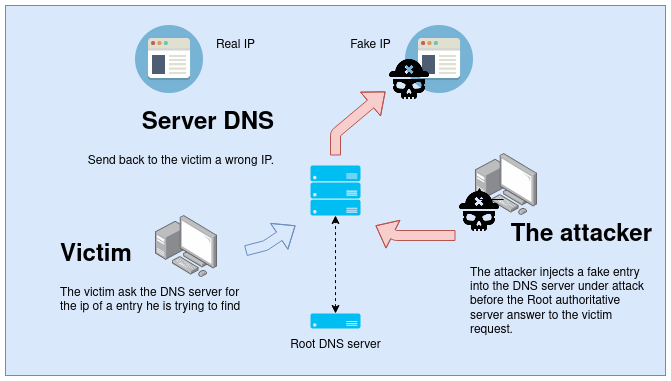
\includegraphics[width=\linewidth]{images/cache_poisoning_scheme.png}
	\caption{Scheme of the attack}
	\label{fig:cache_poisopning_attack}
\end{figure}

\subsection{Question P8 and P9}
The parameters to set inside the \texttt{netwox} command are  set following the tool manual (\ref{conf:netwox_help}):

\inputminted{text}{netwox_help.txt}
\Caption{Netwox help 105}
\label{conf:netwox_help}

In order to perform the attack at first the hacker need to do an ARPspoofing on the internal line using the command \scom{arpspoof -i eth0 -t 20.0.0.1 20.0.0.17} and \scom{arpspoof -i eth0 -t 20.0.0.17 20.0.0.1} then, while the arpspoofing is done the following command need to be entered \scom{sudo netwox 105 --hostname "www.apple.com" --hostnameip "1.2.3.4" --authns "g2.nsa.itscec-lab.ch" --authnsip "86.119.31.49" -ttl 600 --device eth0 --filter "src host 20.0.0.17"  --spoofip "raw"}

After the command is entered, each time a DNS request is send to the DNS server the hacker intercepts the requests and try to fill the DNS server cache with a wrong IP. This mechanism is visible in the following screenshots of wireshark capture (fig \ref{fig:Wireshark_capture}) and in the response obtained to the DNS request which is reported in the listing (\ref{log:nslookup_command})

\begin{figure}[H]
	\centering
	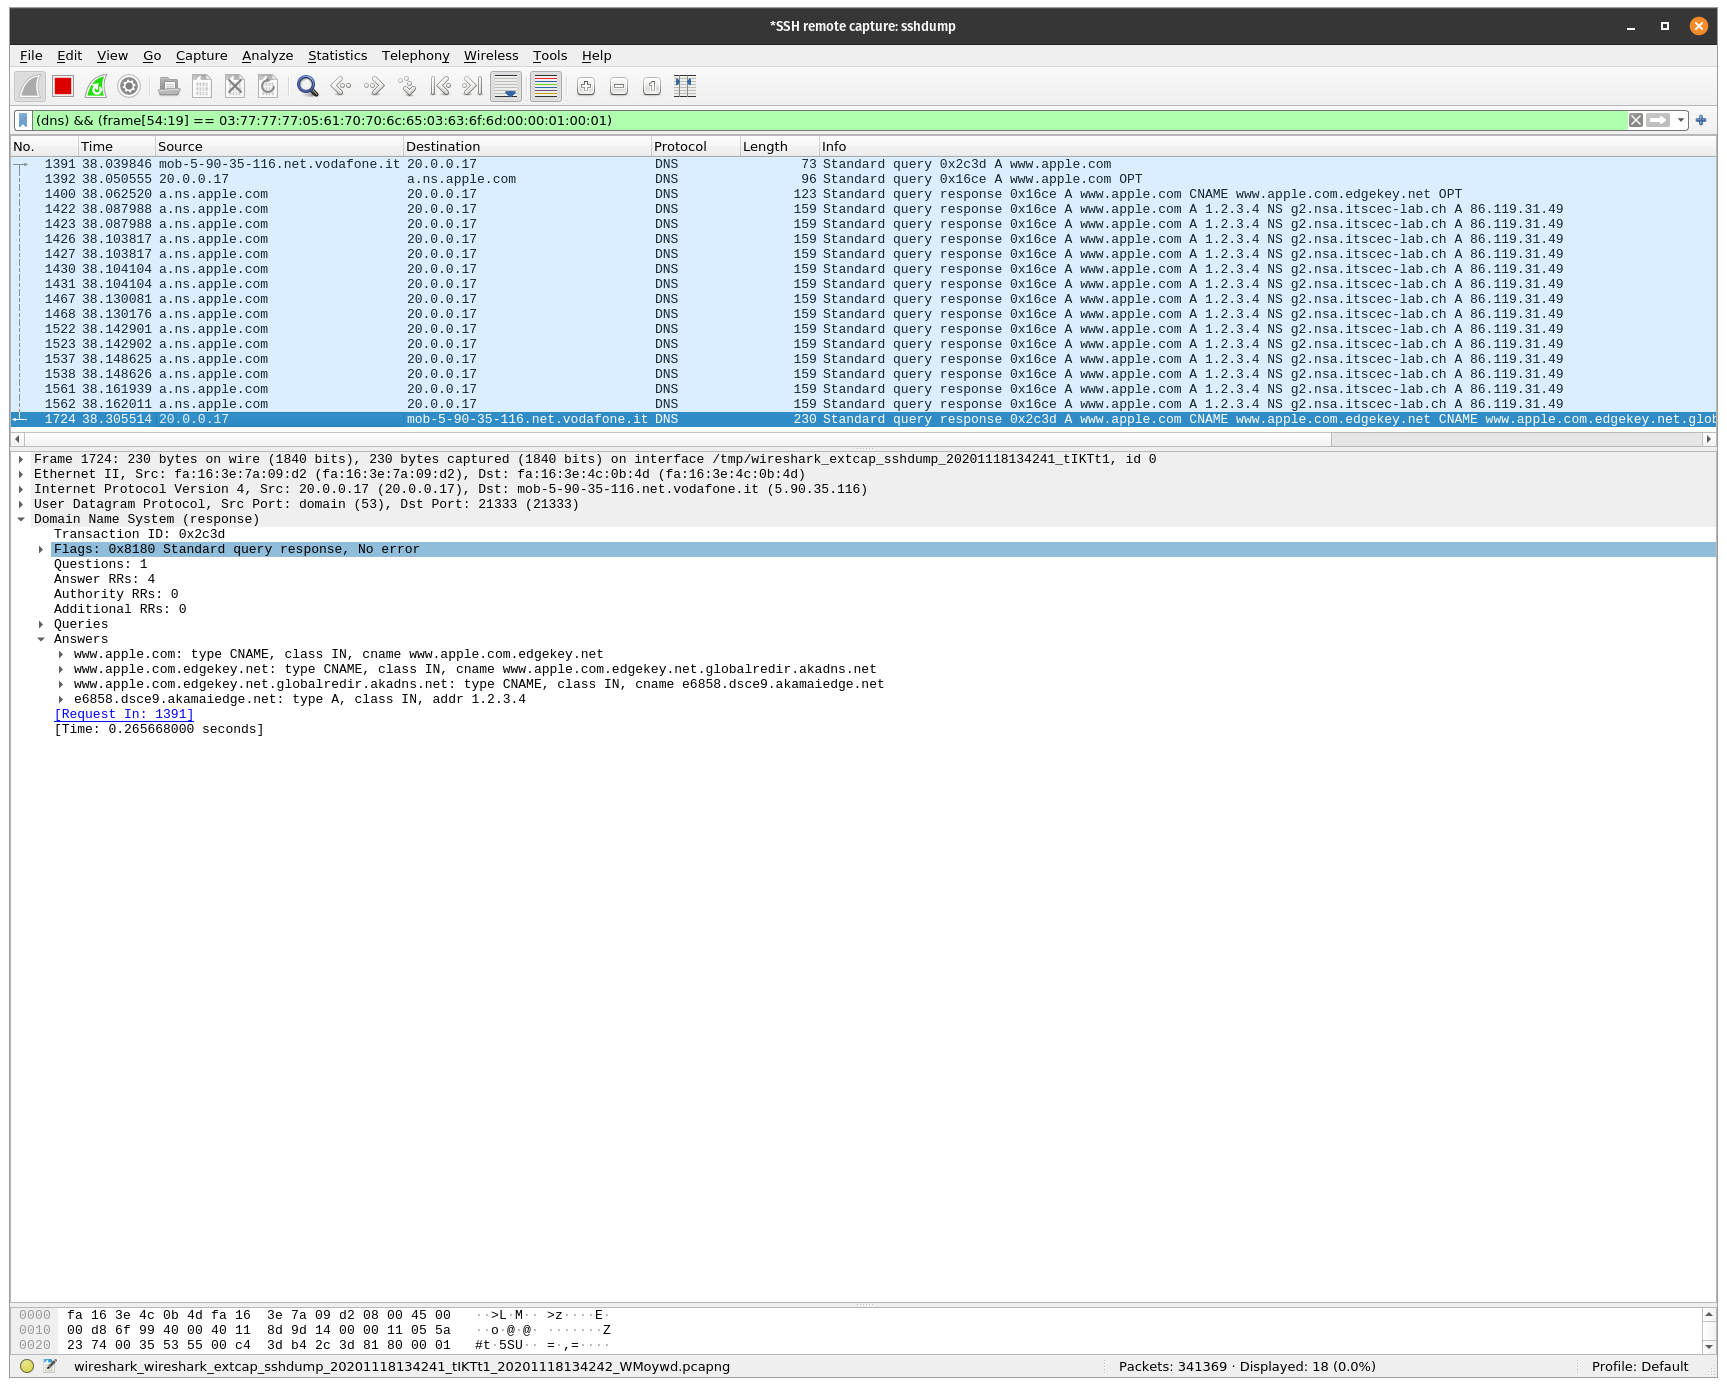
\includegraphics[width=\linewidth]{images/cache_poisoning_wireshark_log.png}
	\caption{Wireshark capture}
	\label{fig:Wireshark_capture}
\end{figure}

\inputminted{text}{cachepoisoning_loca_log.txt}
\Caption{nslookup command on host pc}
\label{log:nslookup_command}


\section{DNSsec configuration}
After following the procedure described in the lab paper the tree of the DNS server is the following

\inputminted{text}{DNSSec_tree.txt}
\Caption{All directories and file in the tree after the complete configuration of the DNSSEC}
\label{log:DNSSec_tree}

\subsection{Question P10}
In order to validate the fact that the DNS server returns the ZONE keys the following command has been entered resulting in the output reported in the listing (\ref{log:DNSSec_zone_keys}) \scom{sudo dig @localhost DNSKEY g2.nsa.itsec-lab.ch -t dnskey}

\inputminted{text}{DNSSec_zone_keys.txt}
\Caption{Check that the server returns the ZONE keys}
\label{log:DNSSec_zone_keys}

\subsection{Question P11}
Following the lab guide A3, it has been tested that the each time a registration is done it is followed by a RRSIG key that contains data element such as Type Covered, Algorithm, Original TTL, Signature Expiration etc. The following listing (\ref{log:DNSSec_RRSIG}) reports the output of the command \scom{sudo dig @localhost DNSKEY g2.nsa.itsec-lab.ch +dnssec}

\inputminted{text}{DNSSec_RRSIG.txt}
\Caption{RRSIG test}
\label{log:DNSSec_RRSIG}

\subsection{Question P12}
In order to complete the chain of trust needed for the DNSSEC then 


\subsection{Question P13}
In order to validate the DNSSEC configuration different tools have been used because some of the options needed in the \Lcode{dig} command are deprecated (\Lcode{+topdown option is deprecated;; +sigchase option is deprecated;; +trusted-key option is deprecated}). Using the website \href{www.dnsviz.net}{dnsviz} a complete check of the DNS chain is possible. In the following images are reported at first the diagram (\ref{fig:dnsviz capture_P1}, \ref{fig:dnsviz capture_P2}, \ref{fig:dnsviz capture_P3}) and then the box reporting the errors (\ref{fig:dnsviz capture_errors}). Due to an error during the configuration the TTL has been set to a very large number (30 day) which is reported as an error because the information in the cache could lead to an error.
\begin{figure}[H]
	\centering
	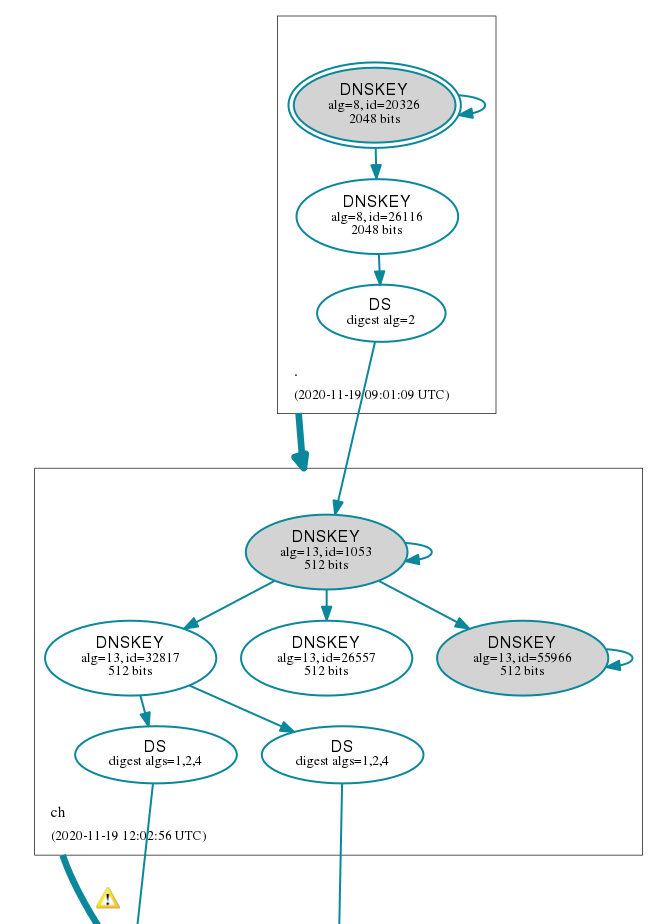
\includegraphics[width=0.7\linewidth]{images/dnspath1.png}
	\caption{dnsviz capture - P1}
	\label{fig:dnsviz capture_P1}
\end{figure}
\begin{figure}[H]
	\centering
	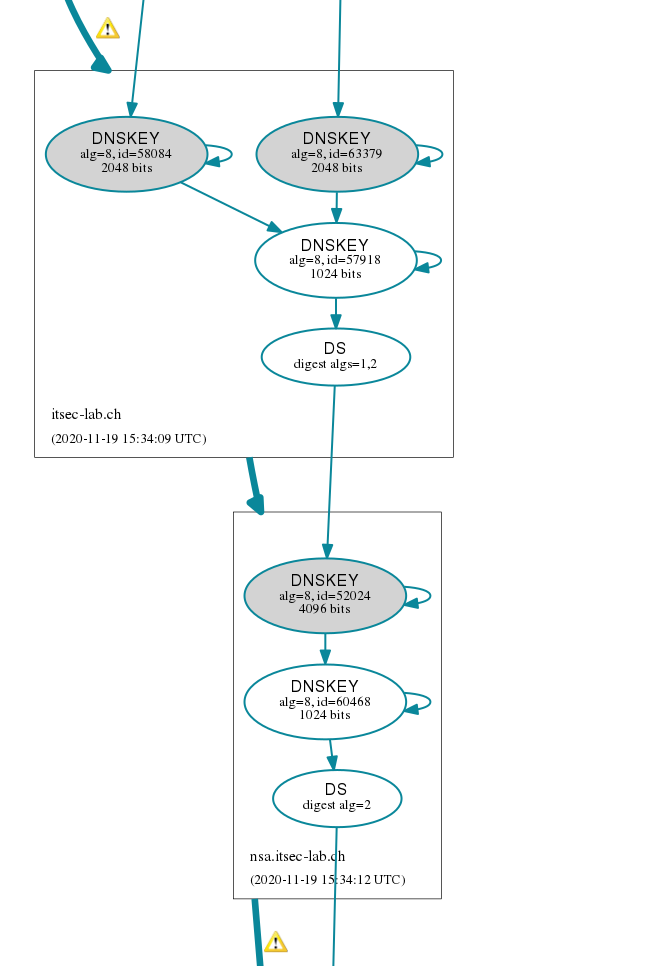
\includegraphics[width=0.7\linewidth]{images/dnspath2.png}
	\caption{dnsviz capture - P2}
	\label{fig:dnsviz capture_P2}
\end{figure}
\begin{figure}[H]
	\centering
	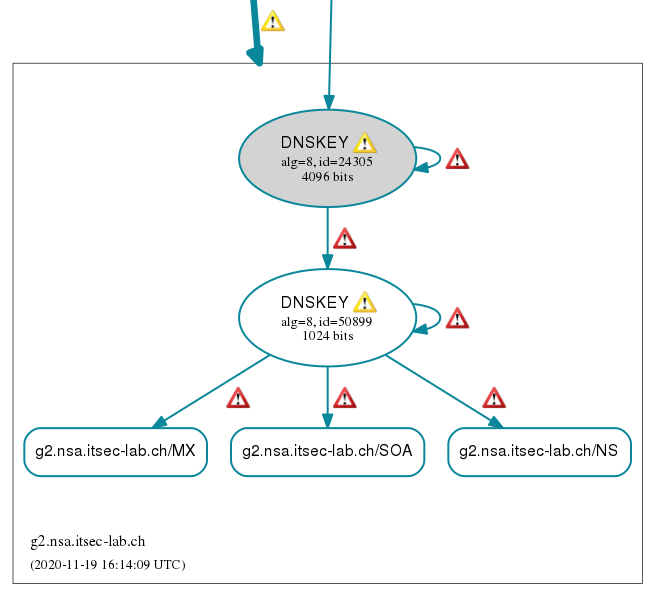
\includegraphics[width=0.7\linewidth]{images/dnspath3.png}
	\caption{dnsviz capture - P3}
	\label{fig:dnsviz capture_P3}
\end{figure}
\begin{figure}[H]
	\centering
	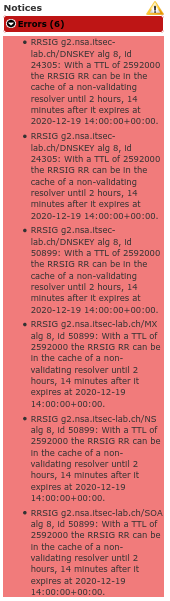
\includegraphics[height=0.5\textheight]{images/errors_dnsviz.png}
	\caption{dnsviz capture -errors}
	\label{fig:dnsviz capture_errors}
\end{figure}

%TODO drill command deprecated options

\subsection{Question P14}

For testing how the server works with a signed page then the following command has been entered \scom{sudo delv +all  @86.119.31.49 www.switch.ch  ANY} and the command output has been

\inputminted{text}{DNSSec_switch_test.txt}
\Caption{www.switch.ch test}
\label{log:DNSSec_switch}

In the output it is visible that at line 2 all the DNS request has been validated.

\subsection{Question P15}
%%%%%%%%%%%%%%%%%%%%%%%%%%%%%%%%%%%%%%%%%%%%%%%%%%%%%%%%%%%%%%%%%%%%%%%%%%%%%%%%


\end{document}
